\section{Introduction}{\label{sec:intro}}
The Internet of Things (IoT) is one of the larger focus areas in today's research of newer computer technology. One definition for IoT is interconnection of computing devices embedded in everyday objects via the Internet, enabling them to send and receive data. According to Cisco, the amount of interconnected devices will be 50 billion by 2020 \cite{ciscoiot:online} \cite{Inter74:online}.

\IEEEPARstart{C}{\MakeLowercase{onstrained}} devices are an essential part of IoT and therefore there is focus on developing lightweight protocols which enables different connectivity models for constrained devices.  
The Constrained Application Protocol (CoAP) \cite{rfc7252} is one of the emerging lightweight application protocols which is designed for machine-to-machine (M2M) applications for use in constrained environments.   

Previously research has been done \cite{interoperabilityChallenge} in the IoTivity framework which operates as a middleware trying to solve interoperability issues in the IoT. Interoperability is about making IoT devices able to connect to any other device or system independent of the used technologies and exchange information as desired, and this area has a potential great economic impact \cite{Unloc34:online}. The IoTivity framework was evaluated against several interoperability requirements and the results from the evaluation shows that device-to-cloud communication within constrained devices is challenging.

IoTivity make use of the CoAP protocol as the only application protocol. 
A new version of the IoTivity framework has been published recently, where the community behind IoTivity has implemented a solution to connect IoT devices to the Cloud \cite{IoTiv3:online}. The solution is based on a newer draft for CoAP \cite{ietf-core-coap-tcp-tls-02} which presents a modified CoAP that runs over TCP instead of UDP, referred to as CoAP over TCP.
The TCP protocol is more complex compared to the UDP protocol and thus it is in general more resource consuming \cite{giannoulis2009tcp}. \figurename{\ref{fig:coapstack}} illustrates the CoAP and the CoAP over TCP stacks.
\begin{figure}[bht]
	\centering
	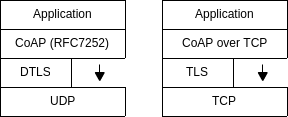
\includegraphics[width=3in]{gfx/coapstack}
	\caption{The CoAP and the CoAP over TCP stacks.}
	\label{fig:coapstack}
\end{figure}

%it is in general not easy to employ on constrained devices. 

% More details from papers about tcp vs udp memory consumption

In this paper we will experimentally evaluate if it is advantageous to use TCP as a transport protocol in CoAP instead of UDP, when CoAP is used for constrained IoT devices.
This evaluation will be done by comparing the two CoAP protocols running on IoTivity, which is the only solution with an implementation of CoAP over TCP. The focus of the evaluation is on the bandwidth and the latency, which both are directly related to the energy consumption. The consequences of using security protocols respectively for UDP (DTLS) and TCP (TLS) are beyond the scope of this research.

The rest of this paper is structured as follows.  Sections \ref{sec:background} and \ref{sec:relatedwork} present the background and related work. Section \ref{sec:experimentsetup} presents the setup of the experiments and section \ref{sec:experimentalresults} provides the experimental results. Section \ref{sec:casestudy} provides a case study based on Arduino.  Section \ref{sec:discussion} discusses the results and section \ref{sec:conclusion} concludes the paper.    
%The rest of this paper is structured as follows.  Section 2 presents the UDP and TCP versions of CoAP protocol. Section 3 provides a qualitative comparison. Section 4 provides a quantitative analytic comparison of the two protocols. Section 5 discusses the results and concludes the paper.     
